\documentclass[11pt, a4paper]{article}

\usepackage[hidelinks]{hyperref} % run first

\usepackage[a4paper, width=14cm]{geometry}

\usepackage[english]{babel}
\usepackage{graphicx}
\graphicspath{ {./figures/} }

\usepackage[]{cleveref} % run last [noabbrev]

\title{The Cambridge Rocketry Simulator User Guide}

\author{Willem Eerland}

\date{\emph{last updated:} \today}

% custom command for folders and files
\newcommand{\loc}[1]{{\footnotesize \textsc{#1}}}

\usepackage{tikz}
\usetikzlibrary{trees}

\tikzstyle{every node}=[draw=black,thick,anchor=west]
\tikzstyle{closed}=[dashed, fill=gray!10]

\begin{document}

\maketitle

\newpage

\tableofcontents

\newpage

\section{Introduction}

This report provides an overview of the various components, and how these can be used to generate rocket trajectories. The program itself is published under the GNU General Public License v3.0 (GPLv3), as the Graphical User Interface (GUI) is taken from an open-source rocket simulator, OpenRocket. The latest version of the Cambridge Rocketry Simulator can be found at \url{https://sourceforge.net/projects/camrocsim/}.

The report starts in \cref{sec:design}, where all parts available for the rocket design are described. This also includes the rocket motor, and the corresponding thrust curve in \cref{subsec:motor}. Next, \cref{sec:simulation} discusses the setting of launch conditions. Finally, \cref{sec:export} explains how the rocket design and launch conditions are used to produce trajectories.

\section{Designing a rocket} \label{sec:design}

% intro
This section describes how a single stage rocket is build. The components in this section are added in the tab \emph{Rocket design}, except the rocket motor, which is added in the tab \emph{Motors \& Configuration}.
%
While there are no restrictions in the software, it is advised that only design with positive stability values are launched (note the stability value in the upper-right corner of the rocket drawing, seen in \cref{fig:tab-design}). When simulating a rocket that is unstable by design, the output trajectories will reflect this.
%
Furthermore, a rocket cannot be launched without a rocket motor. The external parts (nose cone, body tube, transition, and fins) influence the centre of pressure, centre of gravity, and moment of inertia. This while the internal parts (inner tube and bulkhead) only influence the centre of gravity and moment of inertia. Finally, a parachute can be added for a soft landing, and a mass component can simulate instrumentation in the form of a point-mass.
%
By convention the rocket design is built up starting with the most upstream component -- that is -- the nose cone.

\begin{figure}
  \centering
    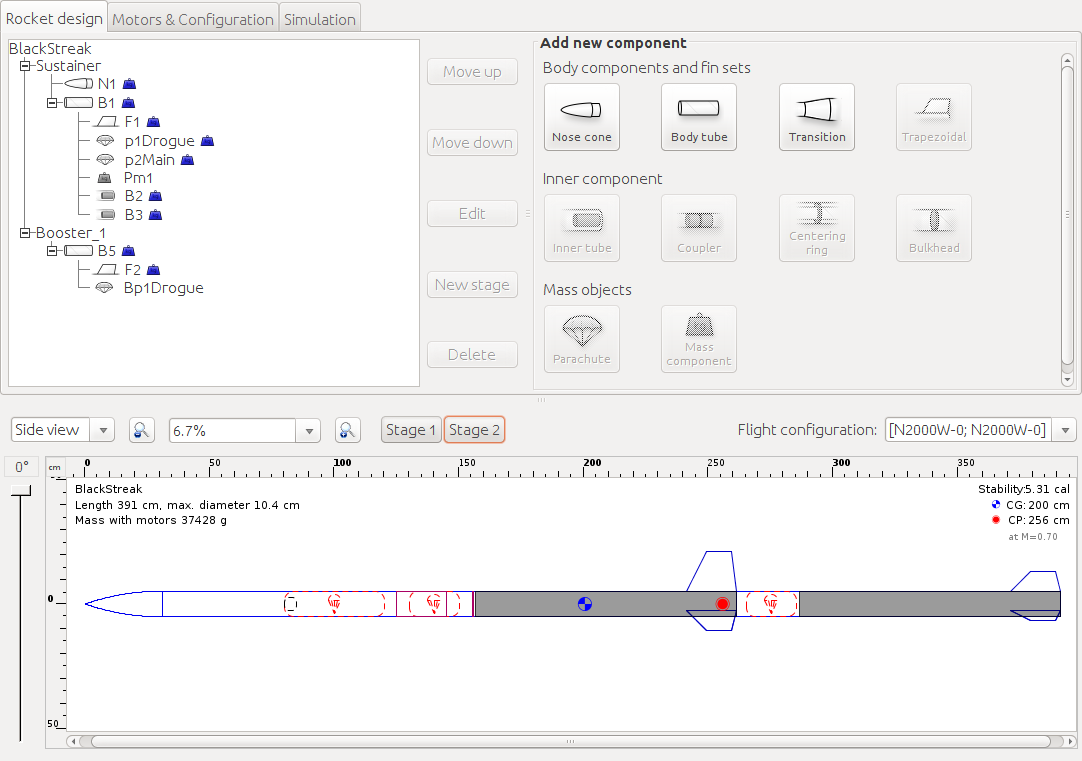
\includegraphics[width=0.9\textwidth]{r-design.png}
  \caption{The \emph{Rocket design} tab.}
  \label{fig:tab-design}
\end{figure}

\subsection{Nose cone}

The nose cone fits at the top of the rocket, and has three options as a shape: ogive, parabolic, and conical. Furthermore, properties such as length, base diameter, thickness, and density. The mass is determined automatically based on the shape and density, but can be overridden in the tab \emph{override}. If desired, a shoulder can be added in the \emph{Shoulder} tab. The shoulder connects the nose cone with the body tube.
%
The centre of pressure is calculated according to the Barrowman equations seen in \cref{table:barrowman}.

\begin{table}[]
\centering
\caption{Barrowman equations used to determine the centre of pressure of the nose cone.}
\label{table:barrowman}
\begin{tabular}{|l|l|}
\hline
\textbf{Shape} & \textbf{Centre of pressure} \\ \hline
Ogive          & 0.466 * length              \\ \hline
Conical        & 2 * length / 3              \\ \hline
Parabolic      & length / 2                  \\ \hline
\end{tabular}
\end{table}

\subsection{Body tube}

Next, the body tube, this is the main body of the rocket and under normal circumstances holds the equipment. If the rocket motor is mounted directly in the body tube, the body tube can be set as a mounting point in the tab \emph{Motor}. Otherwise, when there is an inner tube that holds the rocket motor, the inner tube can be added to the body tube as a sub-component, and be marked as a mounting point there. The body tube has basic parameters such as length, outer diameter, inner diameter, and wall thickness. Naturally the wall thickness is constrained to be consistent with the diameters. In addition to internal sub-components, the body tube also allows for fins as sub-components. The fins are discussed in \cref{subsec:fins}.

\subsection{Transition}

The transition part allows the body tube to change in diameter. It takes the parameters length, fore diameter, aft diameter, and thickness. It can also be used to model a boat-tail.

\subsection{Trapezoidal fins}  \label{subsec:fins}

To increase the stability of the rocket, fins are added to effectively move the centre of pressure. These can only be added as a sub-component of the body tube. Only trapezoidal fins can be added to the model. However, when approximating any other fin-shape, the next best thing to do is to add a trapezoidal fin with an equal surface area. A range of shape parameters can be set, such as: fin rotation, fin cant, root chord, tip chord, heigh, sweep length, sweep angle, and position. Here, the relation between sweep angle and sweep length results in dependence between these parameters. Also the number of fins, thickness, and density can be set. Additionally, in the tab \emph{Fin tabs}, the tabs that connect the fins to the body tube can be added. This has no influence on the aerodynamics, but does influence the mass distribution (centre of gravity and moment of inertia).

\subsection{Inner tube}

The inner tube is an internal component and only influences the centre of gravity and the moment of inertia of the rocket. It has the parameters outer diameter, inner diameter, wall thickness, and length. Here, the outer diameter, inner diameter and wall thickness are connected by dependence. This component can also be used to model a ring that holds other components in place, i.e. a ring is a short inner tube. In the tab \emph{Motor}, the component can be set as a motor mount. In the tab \emph{Radial position}, the radial position can be set. The radial position has an influence on the moment of inertia.

\subsection{Bulkhead}

The bulkhead is an internal component and is very similar to the inner tube, except it is solid all the way through. Because of this, only the parameters diameter, thickness, and density are available.

\subsection{Parachute}

The parachute is required to activate the parachute model. Before deployment, it is modelled as a mass component (\cref{subsec:masscomp}), and takes the parameters packed length, packed diameter, and radial position. After deployment, the parachute dynamic model is activated and wind plays an important role in the simulation. During this phase, the canopy diameter and drag coefficient play the largest role in the descent simulation. The shroud lines only contribute to the mass of the component. The conditions for parachute deployment may be set using \emph{Deploys at}.

\subsection{Mass component} \label{subsec:masscomp}

Any component that has no specific shape can be modelled as a mass component. The properties are similar to the bulkhead, it has a length, diameter, and a mass. It also has a radial position, found in the \emph{Radial position} tab.

\subsection{Rocket motor} \label{subsec:motor}

Finally, the rocket needs a rocket motor to fly. The rocket motor is added to any part that is set as a mount-point, a property available for both the body tube and the inner tube. The rocket motor is added in the top tab \emph{Motors \& Configuration}, seen in \cref{fig:motor}. It takes the shape of a cylinder, and therefore has the properties length, diameter, and a mass.
Where both a `loaded mass' and an `empty mass' are defines. These are respectively the mass of the motor before and after the propellant is burned.
In order to model the thrust as a function of time, a thrust versus time curve needs to be included. This curve has to go through the point $(0,0)$ at the start, and through the point $(t_{end},0)$ at the end. The interface to edit a rocket motor is seen in \cref{fig:motor-edit}.

It is possible to add different configurations to the rocket, with varying rocket engines, and/or parachute deployment.

\begin{figure}
  \centering
    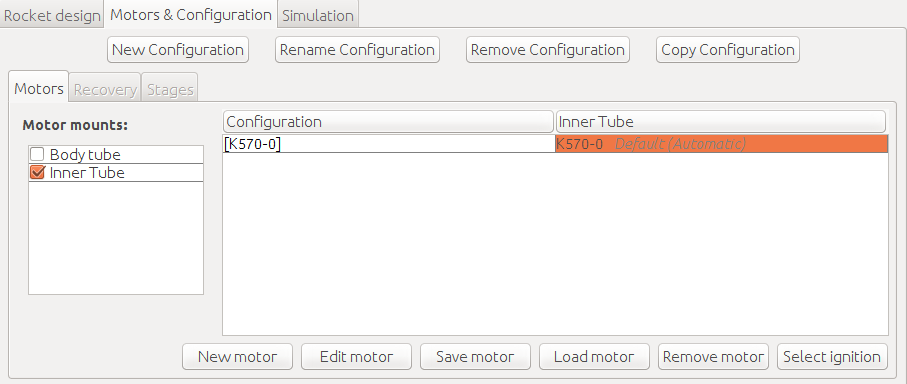
\includegraphics[width=0.9\textwidth]{r-motor.png}
  \caption{The \emph{Motors \& Configuration} tab.}
  \label{fig:motor}
\end{figure}

\begin{figure}
  \centering
    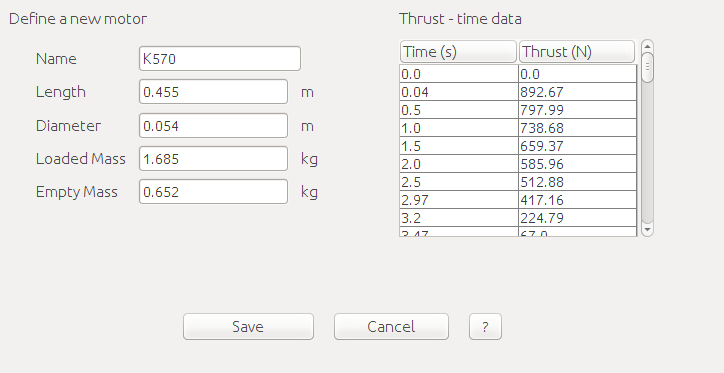
\includegraphics[width=0.9\textwidth]{r-motor-edit.png}
  \caption{Editing a motor via \emph{Edit motor}.}
  \label{fig:motor-edit}
\end{figure}

\section{Setting the launch conditions} \label{sec:simulation}

\begin{figure}
  \centering
    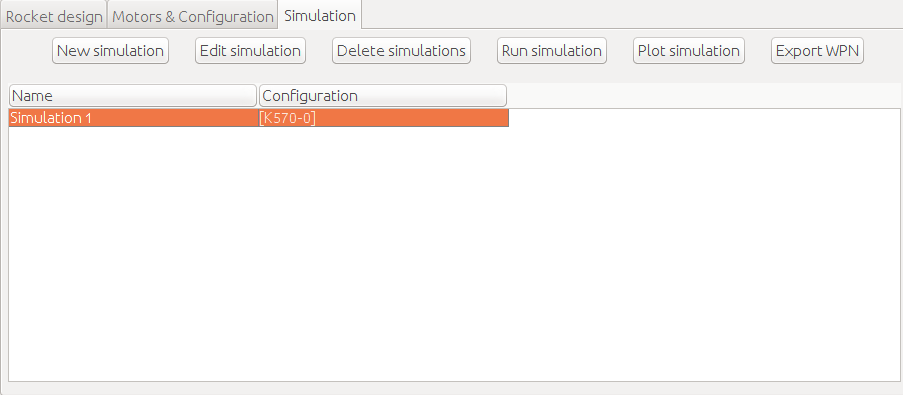
\includegraphics[width=0.9\textwidth]{r-simulation.png}
  \caption{The \emph{Simulation} tab.}
  \label{fig:simulation}
\end{figure}

Once the rocket configuration is complete, the specific launch conditions can be set in the final tab \emph{simulations}, seen in \cref{fig:simulation}. For each simulation it is possible to set-up multiple launch conditions. Each simulation loads a specific atmosphere model, consisting of the wind speed, density, and temperature. And it includes the uncertainties to be taken into account while running the simulation. The options directly available to the user are the launch angle and the thrust. These parameters are available when pressing \emph{Edit simulation}.
The uncertainty in the launch angle allows a range of angles to be evaluated. The value seen in the program provides a measure of maximum deviation from the average.
The uncertainty in the thrust is included as a multiplier to the thrust curve, moving the entire thrust curve up or down by a maximum percentage set in the program. For instance, setting the parameter to $2$ moves the entire curve up or down by a maximum of $2\%$.

While there are other uncertain quantities included in the simulation, such as the drag coefficient, normal coefficient, and centre of pressure. These are included in the file \loc{Uncertainty.xml}, and are not available as user input. These parameters are set based on the confidence in the models used and should not be altered without a good reason.

Finally, it is possible to run the simulation multiple times to explore all possible options. This parameter is called the number of Monte Carlo runs. In theory, there is no minimum number, as only an infinite number of runs assure that all options are covered. In practice, it has a lot to do with the uncertainty in the input domain. The input domain is vastly greater if there is an input angle of plus/minus 10 degrees, or an input angle of plus/minus 1 degree. It is left the user to decide what number of trajectories is sufficient.

\section{Producing trajectories} \label{sec:export}

Once all the parameters are set for a simulation, the process can be started by pressing \emph{Run simulation}. This is in the same tab \emph{simulations}, seen in \cref{fig:simulation}. After pressing \emph{Run simulation}, a window will pop-up to show the progress. The duration of each individual run depends on how far the rocket travels, and the total duration has a linear relation with the number of simulation (the number of Monte Carlo runs). In the background the program \loc{rocketc.exe} takes the files \loc{Uncertainty.xml} and \loc{SimulationInput.xml} and produces the output in \loc{SimulationOutput.xml}. The resulting trajectories can be viewed by pressing \emph{Plot simulation}. The order of producing trajectories after creating a new, or altering an existing design or configuration is:
\begin{enumerate}
\item Run simulation
\item Plot simulation
\end{enumerate}

\section{Producing rocket trajectories via an example rocket}

Producing rocket trajectories with minimal effort is made easy by using one of the example rockets. This section demonstrates how to do exactly that. First, when starting the program, please navigate to and click
\emph{File} \textsc{->} \emph{Open Example...} \textsc{->} \emph{simple-rocket}. A screen will pop-up asking for a description, after which the rocket is displayed as seen in \cref{fig:crs_1}.

\begin{figure}
  \centering
    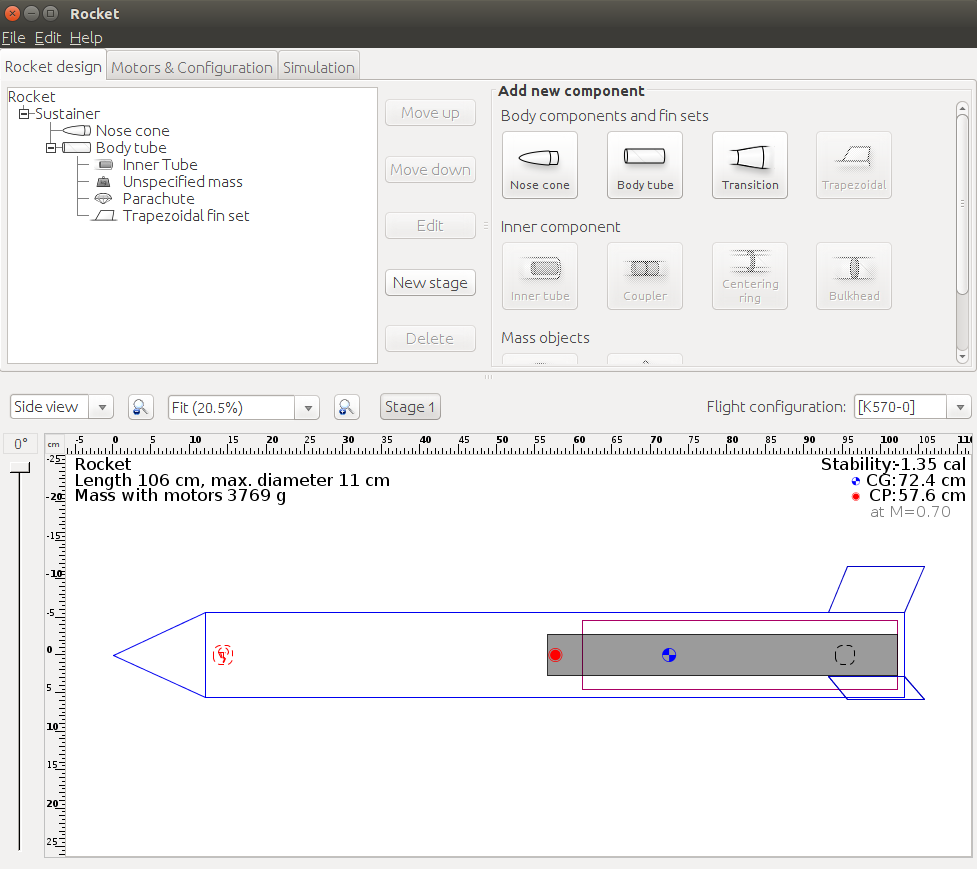
\includegraphics[width=0.9\textwidth]{crs_1_new_rocket.png}
  \caption{Create a new rocket.}
  \label{fig:crs_1}
\end{figure}

This example rocket comes with pre-loaded launch and flight conditions. These are visible by clicking on the \emph{Simulations} tab at the top. This tab has been marked with red in \cref{fig:crs_2}. There are two configurations available, \emph{With wind} and \emph{No wind}. The output trajectories seen in \cref{fig:crs_31,fig:crs_32,fig:crs_33} has been produced by selecting \emph{With wind}, then \emph{Run simulation}, and once this is completed, by pressing \emph{Plot simulation}. All of these buttons have been marked in \cref{fig:crs_2}.

\begin{figure}
  \centering
    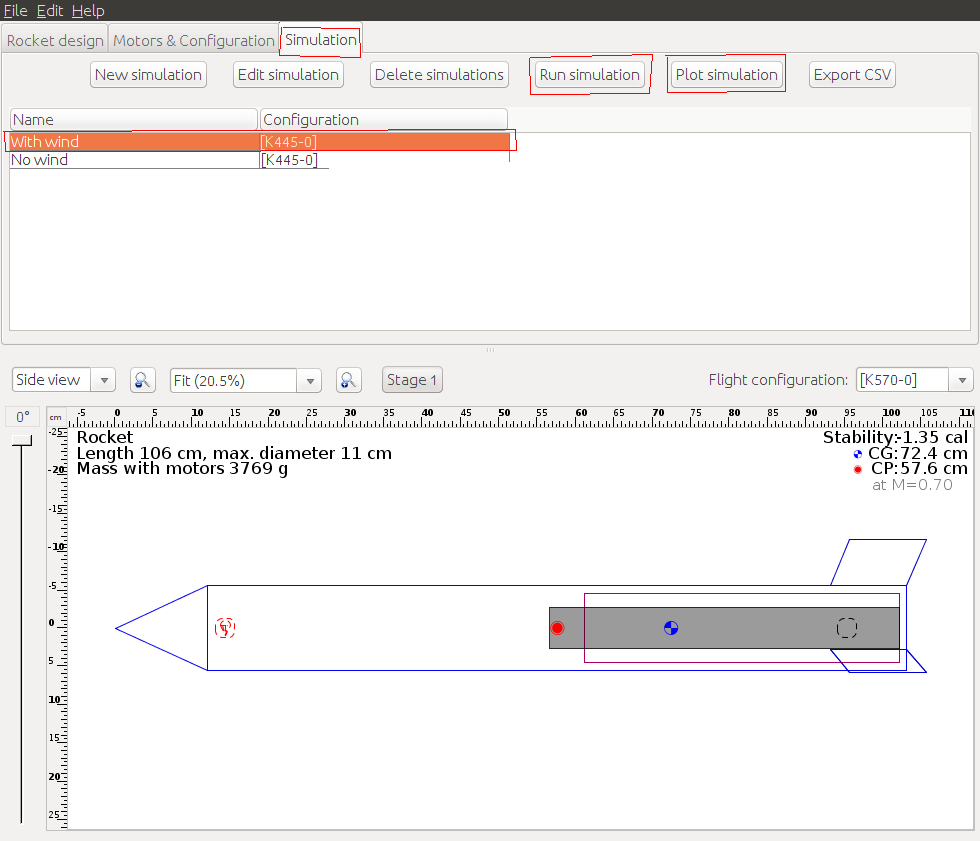
\includegraphics[width=0.9\textwidth]{crs_2_select_simulation.png}
  \caption{Selecting specific conditions and running the simulation.}
  \label{fig:crs_2}
\end{figure}

\begin{figure}
  \centering
    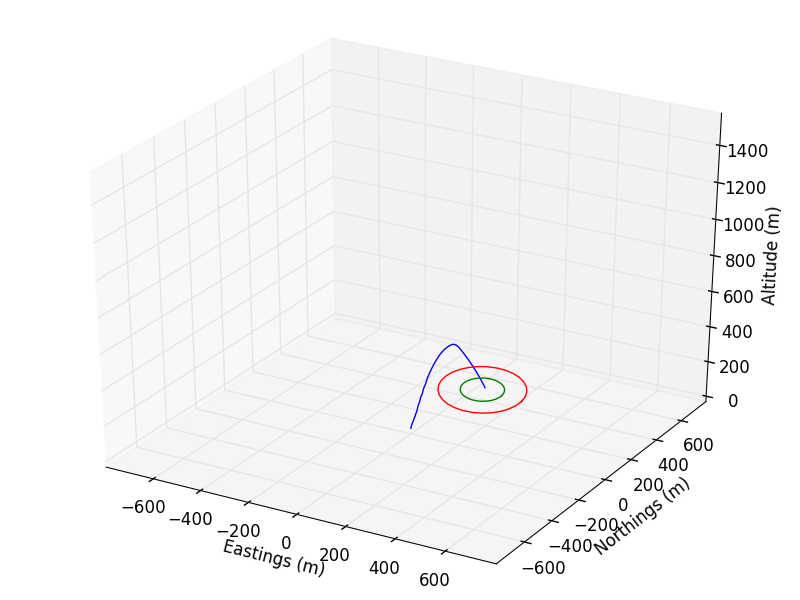
\includegraphics[width=0.9\textwidth]{crs_3_output_1.png}
  \caption{First output figure.}
  \label{fig:crs_31}
\end{figure}

\begin{figure}
  \centering
    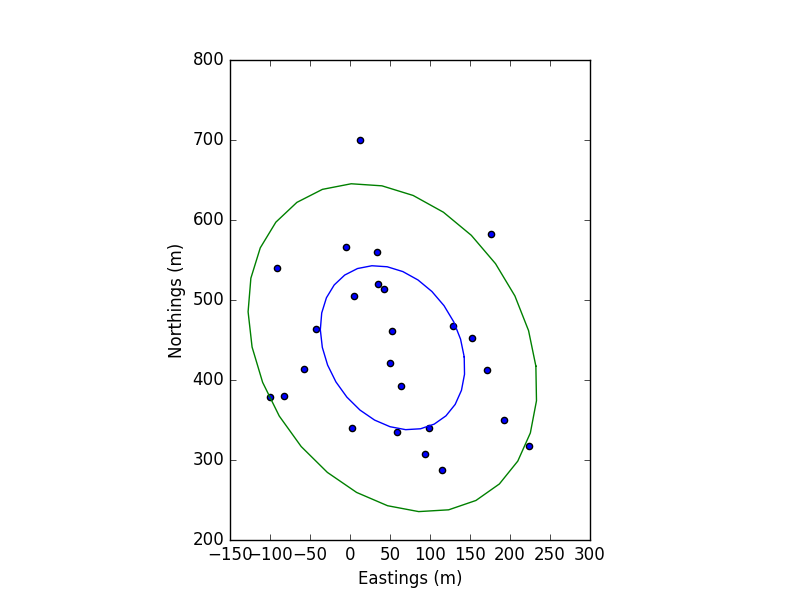
\includegraphics[width=0.9\textwidth]{crs_3_output_2.png}
  \caption{Second output figure.}
  \label{fig:crs_32}
\end{figure}

\begin{figure}
  \centering
    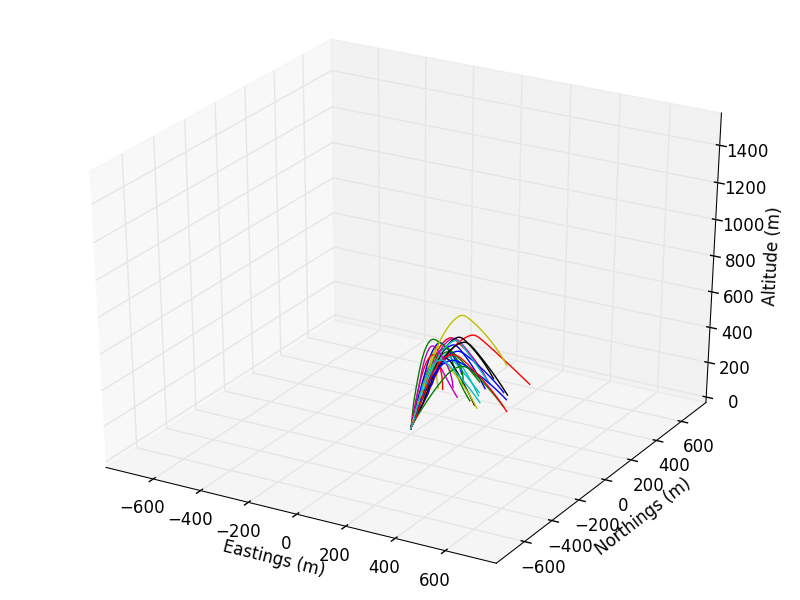
\includegraphics[width=0.9\textwidth]{crs_3_output_3.png}
  \caption{Third output figure.}
  \label{fig:crs_33}
\end{figure}

\section{Command-line access and XML structure}

The Cambridge Rocketry Simulator actually consists of three separate components, where the core, the simulator that takes care of all the physics, takes an XML file as input, and produces an XML file as output. Because of this, the input XML can actually be generated or manipulated manually using a notepad. In a similar fashion, the output XML is also readable by any editor.

% command line access CPP
The simulator core can be invoked by the command line using \loc{./rocketc SimulationInput.xml}, where \loc{SimulationInput.xml} is the default value and can left out, or be replaced by another input XML.
%
In a similar fashion, the Python module, used for plotting the graphs can be invoked with \loc{python FlightPlotter.py}, where the file location is \loc{SimulationOutput.xml} by default. The argument \loc{-f --file} allows pointing to a new location. Furthermore, the arguments \loc{-x --Xaxis} and \loc{-y --Yaxis} allow labeling of the relevant axis, which defaults to an empty string.

% structure xml
The structure belonging to input XML file is visible in \cref{fig:input_simulation_xml}, where due to space restriction the cases {INTAB\_TR} (transition, complete rocket), {INTAB\_BS} (booster stage), {INTAB\_US} (upper stage) are collapsed. They have identical properties, therefore, they are shown as {INTAB\_xx} in \cref{fig:input_simulation_xml_intab_1,fig:input_simulation_xml_intab_2}, which represents the expanded tree for each of these.
% extra information
Information on the expected values of the parameters is available in \cref{tab:input_simulation_xml,tab:input_simulation_xml_1}.

In a similar fashion, the tree of the output XML file is available in \cref{fig:output_simulation_xml}, with a description of the parameters in \cref{tab:output_simulation_xml}.
Finally, the XML file holding the uncertainty information of the input parameters has a tree structure as seen in \cref{fig:output_simulation_xml}, with a description of the parameters in \cref{tab:uncertainty_xml}.

\begin{table}
  \centering
  \caption{InputSimulation.xml}
  \label{tab:input_simulation_xml}
  \begin{tabular}{l p{8cm}}
    \textbf{name} & \textbf{description} \\
    \hline \\
    Time & timestamp \\
    Function & type of simulation; OneStageFlight, TwoStageFlight,  OneStageMonte, or TwoStageMonte \\
    BallisticFailure & deploy parachute \\
    ShortData & include more information in output \\
    NumberOfIterations & monte carlo setting \\
    MaxTimeSpan & maximum number of steps per run \\
    Eastings & start location [m] \\
    Nortings & start location [m] \\
    Altitude & start location [m] \\
    LaunchRailLength & launch rail length [m] \\
    LaunchAzimuth & launch azimuth angle [deg] \\
    LaunchDeclination & launch declination angle [deg] \\
    SeparationTime & timing to release booster stage [s] \\
    IgnitionDelay & activate second stage after separation [s] \\
  \end{tabular}
\end{table}

\begin{table}
  \centering
  \caption{InputSimulation.xml, INTAB\_\emph{xx}}
  \label{tab:input_simulation_xml_1}
  \begin{tabular}{l p{8cm}}
    \textbf{name} & \textbf{description} \\
    \hline \\
    time & timesteps, sets size of all parameters [s] \\
    Thrust & thrust as a function of time [N] \\
    Mass & mass as a function of time [kg] \\
    I\emph{xx} & ineratia as a function of time \\
    CentreOfMass & centre of mass from the nose as a function of time [m] \\
    ThrustDampingCoefficient & thrust damping coefficient as a function of time \\
    AngleOfAttack & angle of attack [deg] \\
    ReynoldsNumber & Reynolds number [-] \\
    CD & drag coefficient as a function of  \\
     & angle of attack and Reynolds number [-] \\
    Cn & normal coefficient [-] \\
    CentreOfPressure & centre of pressure from the nose [m] \\
    Altitude & altitude [m] \\
    Xwind & \emph{x}-direction wind as a function of altitude [m/s] \\
    AtmosphericDensity & atmopsheric density as a function of altitude [kg/$m^3$] \\
    AtmosphericTemperature & temperature as a function of altitude [K] \\
    RocketLength & total length of the rocket [m] \\
    RocketXsectionArea & frontal area of rocket [$m^2$] \\
    ParachuteSwitchAltitude & altitude to activate parachute [m] \\
    ParachuteCDxA & parachute drag coefficient times area [$m^2$] \\
  \end{tabular}
\end{table}

\begin{table}
  \centering
  \caption{OutputSimulation.xml}
  \label{tab:output_simulation_xml}
  \begin{tabular}{l p{8cm}}
    \textbf{name} & \textbf{description} \\
    \hline \\
    Version & identifier for format \\
    Time & identifier for data-set \\
    Function & type of simulation; OneStageFlight, TwoStageFlight,  OneStageMonte, or TwoStageMonte \\
    Number & number of the run \\
    Apogee & x, y, z position of apogee [m] \\
    Landing & x, y, z position of landing [m] \\
    Events & timing of events; activation second stage,  \\
     & apogee, and parachute deployment [s] \\
    AscentTime & timing of apogee [s] \\
    Time & time [s] \\
    Position & x, y, z position as a function of time [m] \\
  \end{tabular}
\end{table}

\begin{table}
  \centering
  \caption{Uncertainty.xml}
  \label{tab:uncertainty_xml}
  \begin{tabular}{l p{11cm}}
    \textbf{name} & \textbf{description} \\
    \hline \\
    Type & \\
    CD & drag coefficient standard deviation, varied as a percentage [-] \\
    CoP & centre of pressure standard deviation, varied as a percentage [-] \\
    CN & normal coefficient standard deviation, varied as a percentage [-] \\
    CDd & primary (first) parachute drag coefficient standard deviation, varied as a percentage [-] \\
    CDp & secondary (any after the first) parachute drag coefficient standard deviation, varied as a percentage [-] \\
    LaunchDeclination & launch declination standard deviation, varied as an absolute value [deg] \\
    Thrust & thrust curve standard deviation, by moving an entire curve up and down [N] \\
    \multicolumn{2}{l}{\textbf{parameters for wind profile} applied in \loc{MonteFy.cpp} } \\
    Mu & average wind speed [m/s] \\
    HScale & altitudes at which to evaluate the wind profile [m] \\
    Sigma & covariance matrix of the basis functions \\
    Eigenvectors & eigenvectors of the covariance matrix Sigma \\
    Eigenvalues & eigenvalues of the covariance matrix Sigma \\
    PHI & basis functions to transform between parameter- and real space \\
  \end{tabular}
\end{table}

\begin{figure}
  \centering
    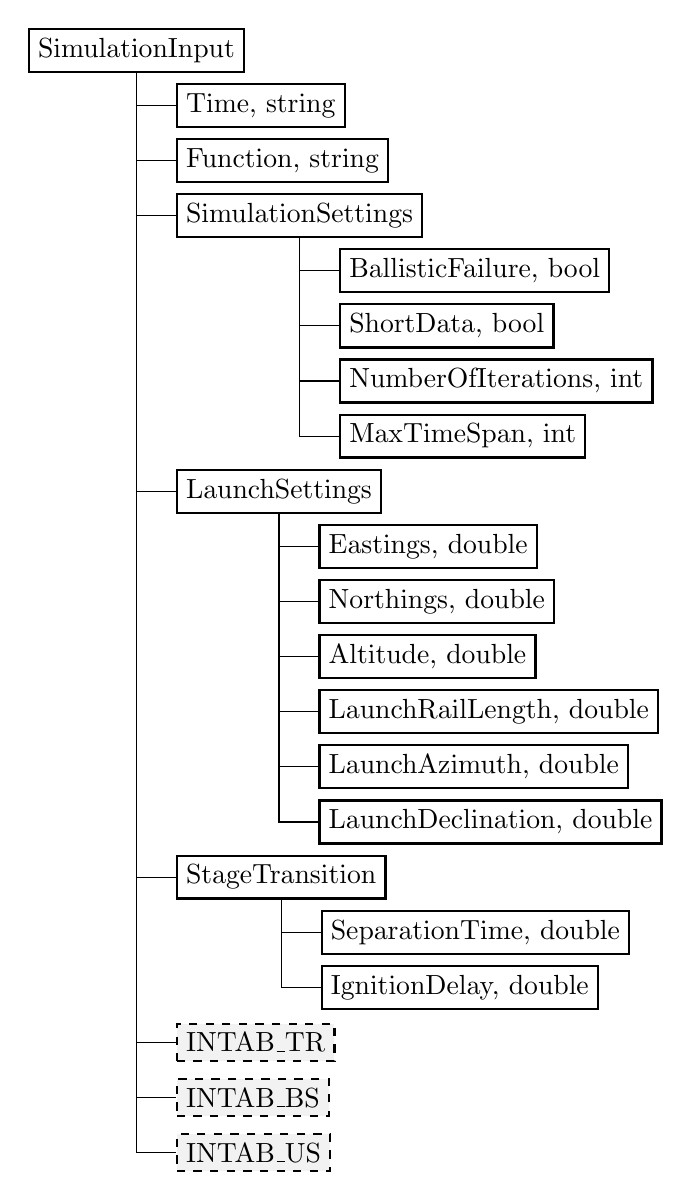
\begin{tikzpicture}[%
      grow via three points={one child at (0.5,-0.7) and
      two children at (0.5,-0.7) and (0.5,-1.4)},
      edge from parent path={(\tikzparentnode.south) |- (\tikzchildnode.west)}]
      \node {SimulationInput}
        child { node {Time, string}}
        child { node {Function, string}}
        child { node {SimulationSettings}
          child { node {BallisticFailure, bool}}
          child { node {ShortData, bool}}
          child { node {NumberOfIterations, int}}
          child { node {MaxTimeSpan, int}}
        }
        child [missing] {}
        child [missing] {}
        child [missing] {}
        child [missing] {}
        child { node {LaunchSettings}
          child { node {Eastings, double}}
          child { node {Northings, double}}
          child { node {Altitude, double}}
          child { node {LaunchRailLength, double}}
          child { node {LaunchAzimuth, double}}
          child { node {LaunchDeclination, double}}
        }
        child [missing] {}
        child [missing] {}
        child [missing] {}
        child [missing] {}
        child [missing] {}
        child [missing] {}
        child { node {StageTransition}
          child { node {SeparationTime, double}}
          child { node {IgnitionDelay, double}}
        }
        child [missing] {}
        child [missing] {}
        child { node [closed] {INTAB\_TR}}
        child { node [closed] {INTAB\_BS}}
        child { node [closed] {INTAB\_US}};
    \end{tikzpicture}
  \caption{SimulationInput.xml}
  \label{fig:input_simulation_xml}
\end{figure}



\begin{figure}
  \centering
    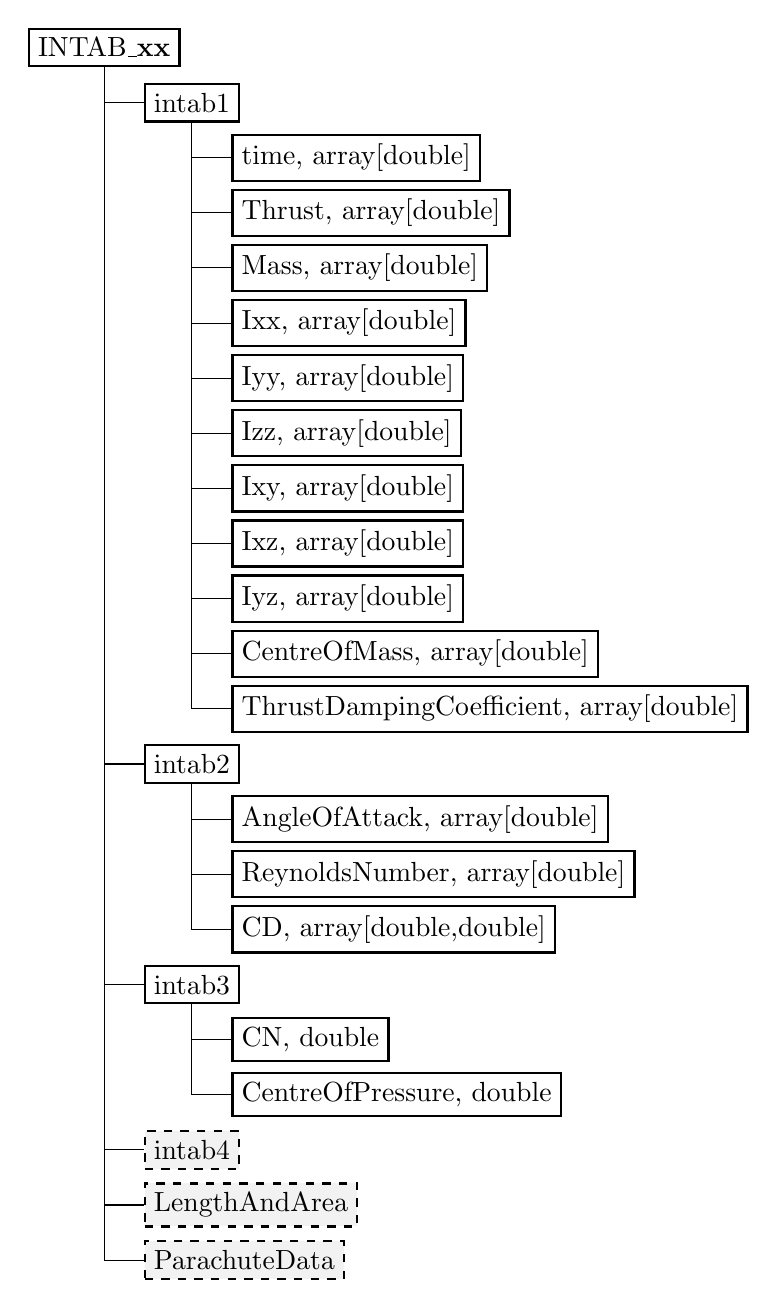
\begin{tikzpicture}[%
      grow via three points={one child at (0.5,-0.7) and
      two children at (0.5,-0.7) and (0.5,-1.4)},
      edge from parent path={(\tikzparentnode.south) |- (\tikzchildnode.west)}]
      \node {INTAB\_\textbf{xx}}
          child { node {intab1}
            child { node {time, array[double]}}
            child { node {Thrust, array[double]}}
            child { node {Mass, array[double]}}
            child { node {Ixx, array[double]}}
            child { node {Iyy, array[double]}}
            child { node {Izz, array[double]}}
            child { node {Ixy, array[double]}}
            child { node {Ixz, array[double]}}
            child { node {Iyz, array[double]}}
            child { node {CentreOfMass, array[double]}}
            child { node {ThrustDampingCoefficient, array[double]}}
          }
          child [missing] {}
          child [missing] {}
          child [missing] {}
          child [missing] {}
          child [missing] {}
          child [missing] {}
          child [missing] {}
          child [missing] {}
          child [missing] {}
          child [missing] {}
          child [missing] {}
          child { node {intab2}
            child { node {AngleOfAttack, array[double]}}
            child { node {ReynoldsNumber, array[double]}}
            child { node {CD, array[double,double]}}
          }
          child [missing] {}
          child [missing] {}
          child [missing] {}
          child { node {intab3}
            child { node {CN, double}}
            child { node {CentreOfPressure, double}}
          }
          child [missing] {}
          child [missing] {}
          child { node [closed] {intab4}}
          child { node [closed] {LengthAndArea}}
          child { node [closed] {ParachuteData}};
    \end{tikzpicture}
  \caption{SimulationInput.xml}
  \label{fig:input_simulation_xml_intab_1}
\end{figure}

\begin{figure}
  \centering
    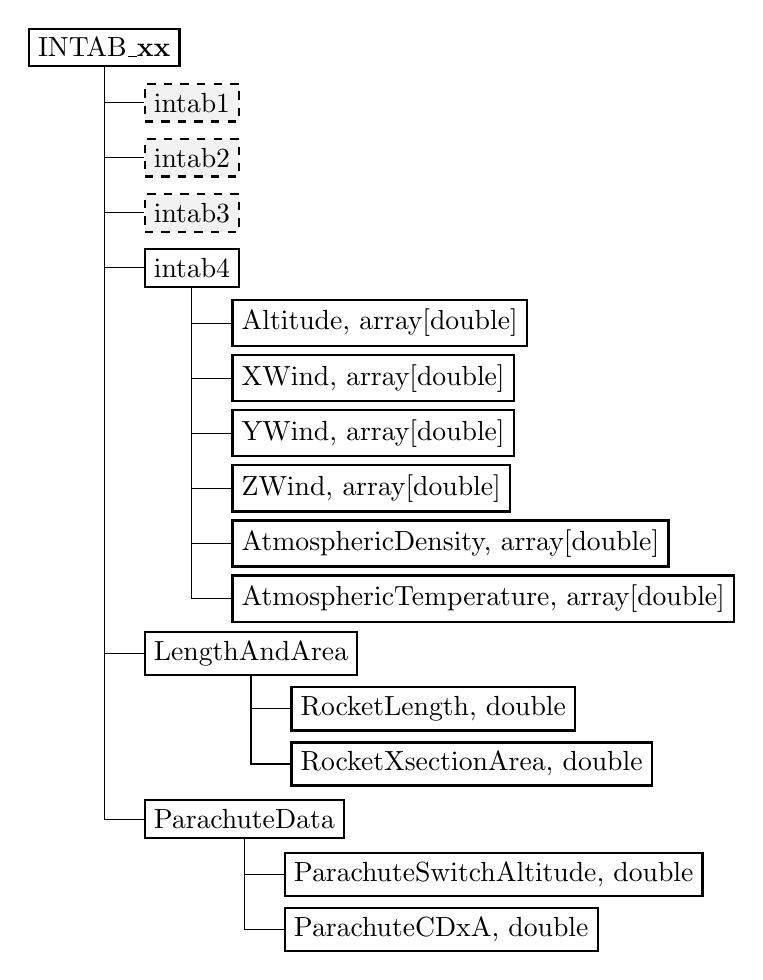
\begin{tikzpicture}[%
      grow via three points={one child at (0.5,-0.7) and
      two children at (0.5,-0.7) and (0.5,-1.4)},
      edge from parent path={(\tikzparentnode.south) |- (\tikzchildnode.west)}]
      \node {INTAB\_\textbf{xx}}
          child { node [closed] {intab1}
          }
          child { node [closed] {intab2}
          }
          child { node [closed] {intab3}
          }
          child { node {intab4}
            child { node {Altitude, array[double]}}
            child { node {XWind, array[double]}}
            child { node {YWind, array[double]}}
            child { node {ZWind, array[double]}}
            child { node {AtmosphericDensity, array[double]}}
            child { node {AtmosphericTemperature, array[double]}}
          }
          child [missing] {}
          child [missing] {}
          child [missing] {}
          child [missing] {}
          child [missing] {}
          child [missing] {}
          child { node {LengthAndArea}
            child { node {RocketLength, double}}
            child { node {RocketXsectionArea, double}}
          }
          child [missing] {}
          child [missing] {}
          child { node {ParachuteData}
            child { node {ParachuteSwitchAltitude, double}}
            child { node {ParachuteCDxA, double}}
          }
          child [missing] {}
          child [missing] {};
    \end{tikzpicture}
  \caption{SimulationInput.xml}
  \label{fig:input_simulation_xml_intab_2}
\end{figure}

\begin{figure}
  \centering
    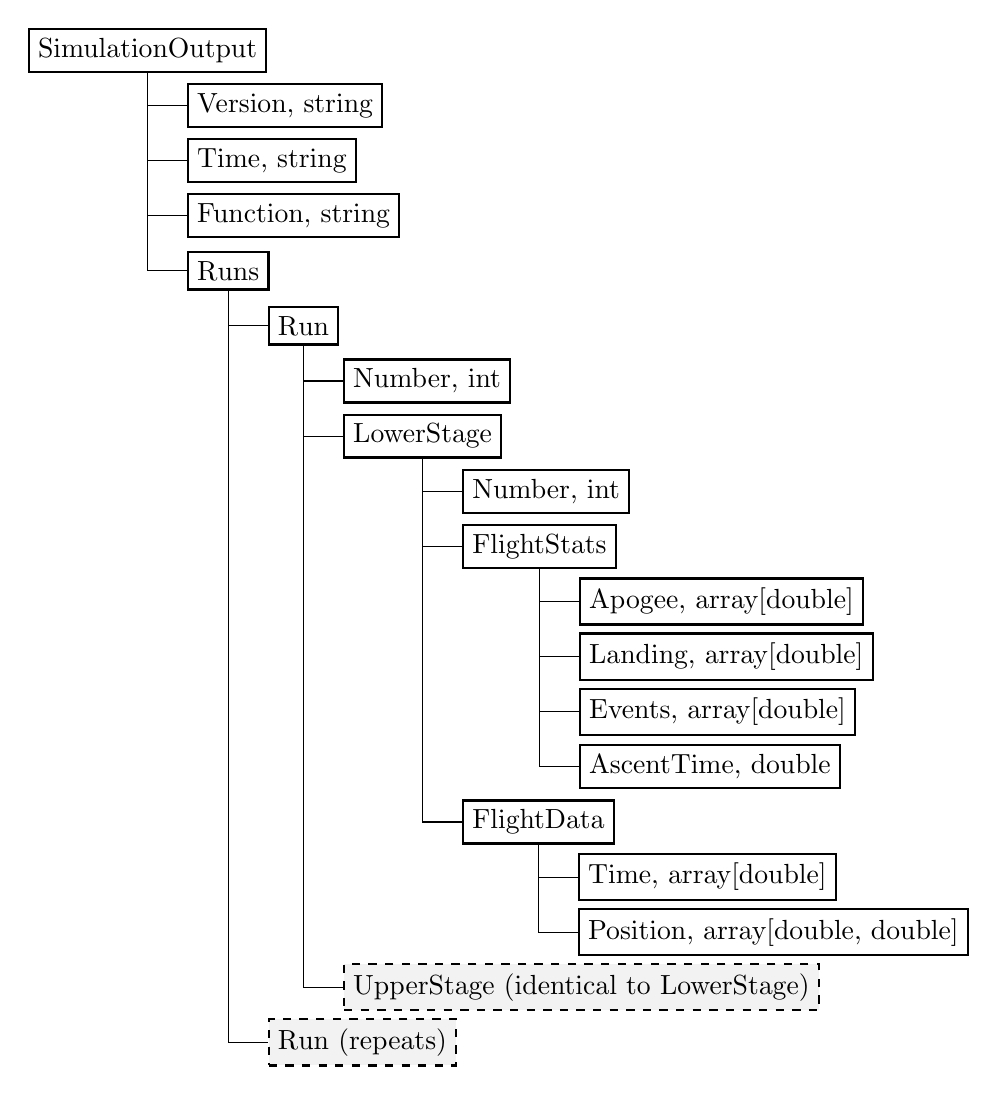
\begin{tikzpicture}[%
      grow via three points={one child at (0.5,-0.7) and
      two children at (0.5,-0.7) and (0.5,-1.4)},
      edge from parent path={(\tikzparentnode.south) |- (\tikzchildnode.west)}]
      \node {SimulationOutput}
        child { node {Version, string}}
        child { node {Time, string}}
        child { node {Function, string}}
        child { node {Runs}
          child { node {Run}
            child { node {Number, int}}
            child { node {LowerStage}
              child { node {Number, int}}
              child { node {FlightStats}
                child { node {Apogee, array[double]}}
                child { node {Landing, array[double]}}
                child { node {Events, array[double]}}
                child { node {AscentTime, double}}
              }
              child [missing] {}
              child [missing] {}
              child [missing] {}
              child [missing] {}
              child { node {FlightData}
                child { node {Time, array[double]}}
                child { node {Position, array[double, double]}}
              }
              child [missing] {}
              child [missing] {}
            }
            child [missing] {}
            child [missing] {}
            child [missing] {}
            child [missing] {}
            child [missing] {}
            child [missing] {}
            child [missing] {}
            child [missing] {}
            child [missing] {}
            child { node [closed] {UpperStage (identical to LowerStage)}}
          }
          child [missing] {}
          child [missing] {}
          child [missing] {}
          child [missing] {}
          child [missing] {}
          child [missing] {}
          child [missing] {}
          child [missing] {}
          child [missing] {}
          child [missing] {}
          child [missing] {}
          child [missing] {}
          child {node [closed] {Run (repeats)}}
        };
    \end{tikzpicture}
  \caption{SimulationOutput.xml}
  \label{fig:output_simulation_xml}
\end{figure}

\begin{figure}
  \centering
    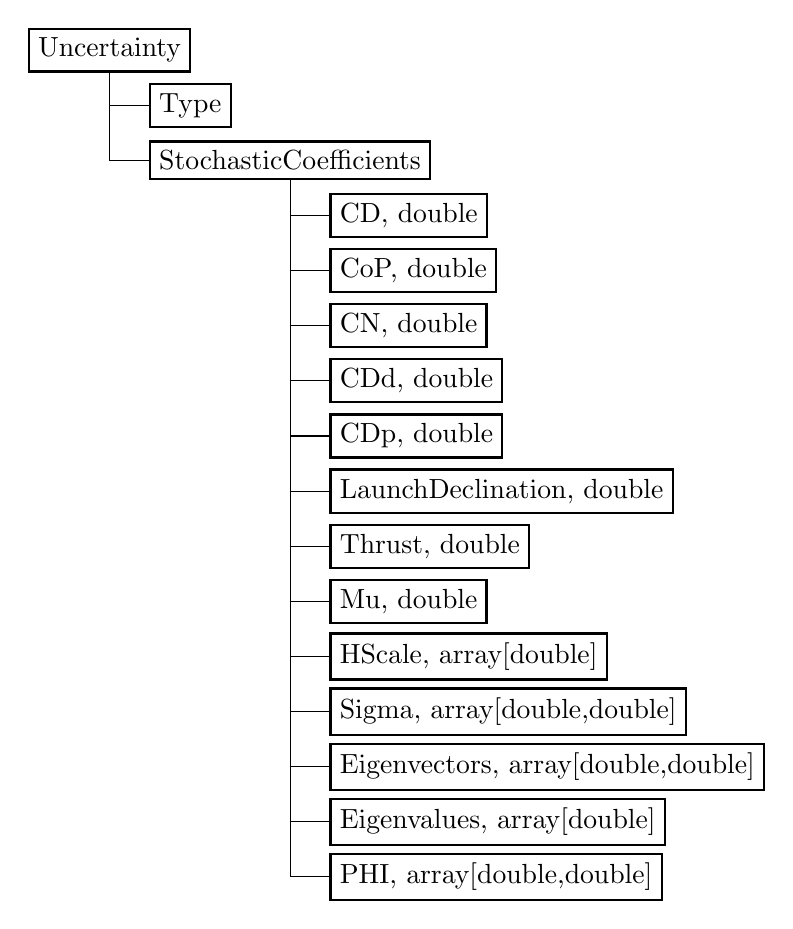
\begin{tikzpicture}[%
      grow via three points={one child at (0.5,-0.7) and
      two children at (0.5,-0.7) and (0.5,-1.4)},
      edge from parent path={(\tikzparentnode.south) |- (\tikzchildnode.west)}]
      \node {Uncertainty}
        child { node {Type}}
        child { node {StochasticCoefficients}
          child { node {CD, double}}
          child { node {CoP, double}}
          child { node {CN, double}}
          child { node {CDd, double}}
          child { node {CDp, double}}
          child { node {LaunchDeclination, double}}
          child { node {Thrust, double}}
          child { node {Mu, double}}
          child { node {HScale, array[double]}}
          child { node {Sigma, array[double,double]}}
          child { node {Eigenvectors, array[double,double]}}
          child { node {Eigenvalues, array[double]}}
          child { node {PHI, array[double,double]}}
        };
    \end{tikzpicture}
  \caption{Uncertainty.xml}
  \label{fig:uncertainty_xml}
\end{figure}

\end{document}
